\section{Introduction}
%PUT IT ON ZENODO
The Sun's activity in April 2022 increased drastically compared to earlier that year. Indeed, 12 out of the 50 strongest Earth directed solar flares of the year were detected in that only month\footnote{\url{https://www.spaceweatherlive.com/en/solar-activity/top-50-solar-flares/year/2022.html}}. Moreover, 159 coronal mass ejections (CMEs) were detected by the LASCO instrument aboard SOHO in April 2022\footnote{\url{https://www.sidc.be/cactus/catalog.php}}. This is a $\sim$ 79\% increase compared to the average of the 5 precedent months. Combined with an elongation of Venus near its maximal value of 47.8°, the observation conditions of this planet in the high-energy ranges were close to optimal. This report presents the approach used to recover the X-ray flux from a moving object, Venus, in the 3-10 keV energy range using the data from the JEM-X instrument aboard the \textit{INTEGRAL} telescope. The values detected from Venus' position are then compared to the Sun's activity during that period.

This \textbf{Introduction }section first presents the telescope and instrument used. Then the data retrieving method using the \textit{Online Data Analysis - Application Programming interface} (\texttt{ODA-API}) of \textit{INTEGRAL} is described. The main channels of X-ray emission of planets are presented.

The \textbf{Observation, data analysis and methods} section shows the steps in the selection of the data, the criteria, assumptions and models used. This comprises how the solar events were obtained and analysed.

The \textbf{Results} section presents the results of the Venus fluxes using three different methods. The fluxes are then timewise compared with the solar fluxes. A solar event locator is presented using the \texttt{Sunpy} library.

Finally, the obtained results are thoroughly examined and interpreted in the \textbf{Discussion} section. The significance and implications of the findings are analysed. Furthermore, future research directions are proposed, highlighting potential avenues for further investigation. 

\textbf{Annex A} provides additional figures on the models used. \textbf{Annex B} lists the different useful resources affiliated to this project.

\subsection{INTEGRAL telescope}
%talk about what is a scw and put links to some of the integral stuff. Otherwise ref to all the links in the git.
The INTErnational Gamma-RAy Laboratory (\textit{INTEGRAL}), launched in 2002 on an elliptic orbit around Earth, is ESA's successor mission to the Cos-B and CGRO telescopes. For 19 years, it has been producing complete maps of the sky in the soft-gamma ray and X-ray sources (keV-MeV range) thanks to its four main instruments: IBIS imager (15 keV-10 MeV), SPI spectrometer (20 keV-8 MeV with a 2 keV spectral resolution at 1.33 MeV), JEM-X X-ray monitor and the OMC optical camera (V-band).
    
    \begin{figure}[H]
        \centering
        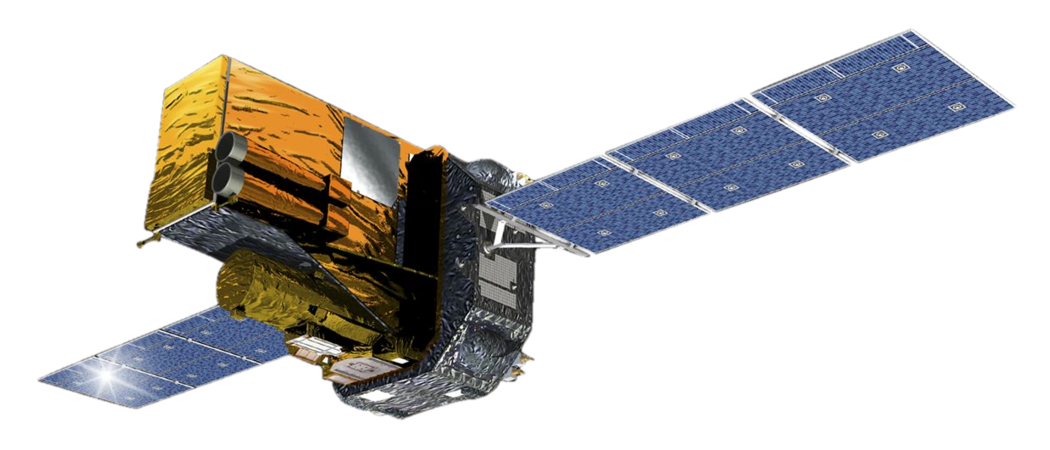
\includegraphics[width = 8cm]{report/Figures/intro/INTEGRAL_spacecraft_model.png}
        \caption{Artist's representation of the \textit{INTEGRAL} telescope.}
        \label{integral}
    \end{figure}
    
        \subsection{JEM-X detector}
        The Joint European Monitor for X-rays (JEM-X) is a complementary detector on-board the \textit{INTEGRAL} telescope. It is primarily used to support the IBIS and SPI instruments in the lower energies for the studies of $\gamma$-ray and X-ray sources. It can however also provide independant scientific results for soft-spectra sources that could be serendipitously detected in the field-of-view(FOV) of the detector. This is the case for Venus here.
        % add a table of jemx parameter and performance. See table 1 of osa_um_jemx.pdf
        The characteristics of JEM-X can be found on \textbf{Tab.} \ref{jemx_perf}. \textbf{Fig.} \ref{jemx}a shows a splitted view of the different constituents of the instrument. \textbf{Fig.} \ref{jemx}b is a top view representation of the coded mask of JEM-X. The instrument actually consists of two of these coded-aperture mask telescope units: JEM-X1 and JEM-X2. Each unit is composed of three parts: the detector, the electronics and the coded mask. For this study, only JEM-X2 data were used.

        The detector of each JEM-X unit consists of a microstrip gas chamber (90\% xenon and 10\% methane at 1.5 bar). The incoming photons are absorbed in the xenon gas by photo-electric absorption and the resulting ionization cloud is then amplified in an avalanche of ionisations by the strong electric field near the microstrip anodes\cite{2020ISDCManual}.

        High-energy electromagnetic radiations cannot be observed using lenses or mirrors. Instead, patterns of materials opaque to the observed wavelengths called \textit{coded-aperture masks} are used. An illustration is shown on \textbf{Fig.} \ref{jemx}b. By blocking the incoming radiation in a pre-determined pattern using mask elements, the image of the source observed casts a shadow on the detector. Reconstruction algorithms are then used to find the position of the source and its intensity\footnote{See \url{https://asd.gsfc.nasa.gov/archive/cai/coded_intr.html\#section2} for details and \cite{Dicke1968SCATTER-HOLERAYS}}. The resolution of the mask is defined by the mask height above the detector and the mask element size. For JEM-X, these a respectively 3.4m and 3.3mm\cite{2020ISDCManual}.

        %explain detector(in osa_um_jemx.pdf) + coded mask(find on internet), don't forget to say that above 5°, the response is too low so the query is only done within 5°.

        \begin{table}[H]
        \centering
        \begin{tabular}{@{}lc@{}}
        \toprule
        \multicolumn{2}{c}{\textbf{JEM-X Performance parameters}} \\ \midrule
        Energy range [keV]                  & 3 - 35              \\
        Detector area/effective [cm$^2$]    & 500/125             \\
        Energy resolution                   & 1.3 keV @ 10 keV    \\
        Field-of-View (FoV)                 & 4.8° (Fully coded)  \\
        Angular resolution (FWHM) [arcmin]  & 3                   \\ 
        Pixel size [arcmin]                 & 1.56               
        \end{tabular}
        \caption{JEM-X key performance parameters. See \href{https://www.cosmos.esa.int/web/integral/instruments-jemx}{here} for more details.}
        \label{jemx_perf}
        \end{table}
        
        \begin{figure}[H]
        \centering
        \begin{subfigure}{.45\textwidth}
            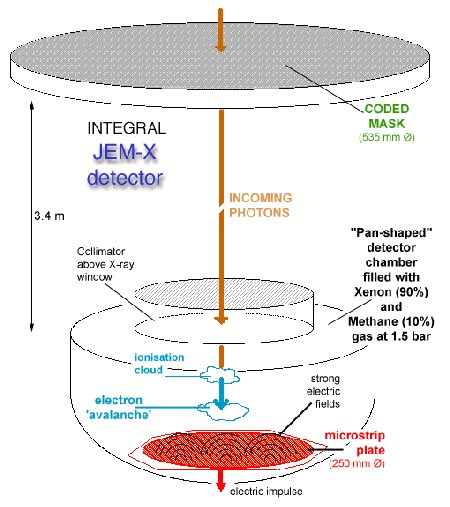
\includegraphics[width=\textwidth]{report/Figures/intro/jem_x_funct_diagram.jpg}
        \end{subfigure}%
        \hspace{1em}-
        \begin{subfigure}{.45\textwidth}
            \centering
            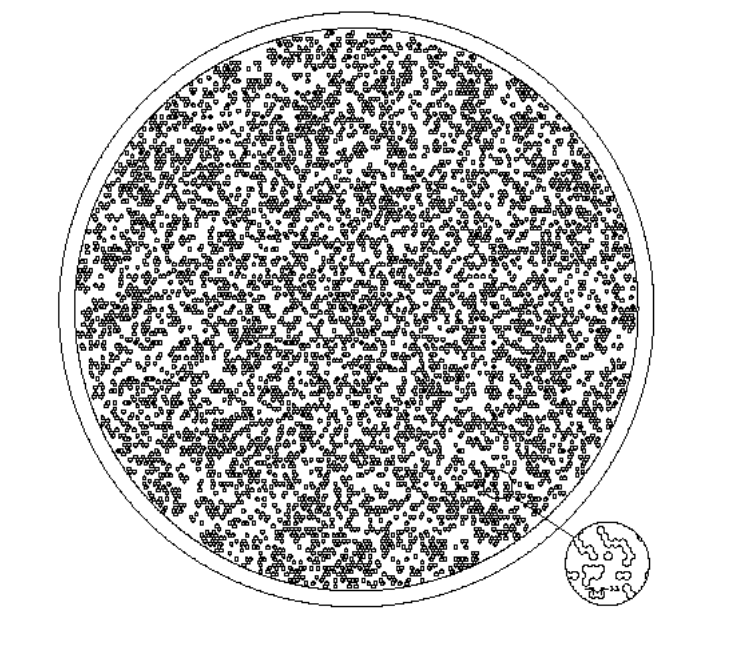
\includegraphics[width=\textwidth]{report/Figures/intro/jemx_coded_mask.png}
        \end{subfigure}
        \caption{(left) Schematic diagram of the different JEM-X constituents. (right) JEM-X's coded mask.}
        \label{jemx}
        \end{figure}
    
    \subsection{\texttt{ODA-API}}

    Spanning more than nineteen years of nearly continuously taken data, the \textit{INTEGRAL} archives contain information on a large number of sources. The mission was initially planned to operate only for five years and the data sets generated were supposed to stay relatively small. But common to scientific space missions, the life of the telescope was extended as long as it stayed functional. The data analysis pipelines for all instruments uses the Offline Science Analysis (OSA) software distributed by the \textit{INTEGRAL} Science Data Centre (ISDC). This software was optimised for the initial mission and the only solution for data processing before \texttt{ODA-API} was via a local installation of OSA on a user computer. Given the amount of data generated since then, the data processing resources now require a significant amount of computing resources. This is why the \texttt{ODA} was developed. It provides an online \textit{INTEGRAL} data analysis system using high-performance and cloud computing technologies accessible through a web browser via the ODA website\footnote{\url{https://www.astro.unige.ch/mmoda/}} or through an API from e.g. a \texttt{Jupyter} notebook by querying the required parameters (see \textbf{List.} \ref{dict} for an example). The \texttt{ODA-API} was used in this study to retrieve the data from the \textit{INTEGRAL} archives.

    \subsection{HEASARC and \textit{INTEGRAL} Science Window Data}

    The High Energy Astrophysics Science Archive Research Center (HEASARC)\footnote{\url{https://heasarc.gsfc.nasa.gov/}} is the primary archive for space missions studying high energy electromagnetic radiations phenomena. The \textit{INTEGRAL} data is queried from the ISDC data servers using the \texttt{astroquery.heasarc} Python interface\footnote{\url{https://astroquery.readthedocs.io/en/latest/heasarc/heasarc.html\#using-alternative-heasarc-servers}}.

    \textit{INTEGRAL}'s activities are splitted into different categories called \textit{windows}. \textit{Science windows} (scw) are what interest us here. Quoting the ISDC, they are continuous time intervals during which all data acquired by the INTEGRAL instruments result from a specific spacecraft attitude orientation state. Scws have different parameters among which their observation identifier (Obs\textunderscore ID) which is a sequence of 11 digits identifying each scw\footnote{See \url{https://heasarc.gsfc.nasa.gov/W3Browse/integral/intscw.html} for more details.}.
    

    \subsection{X-ray emission of planets: the case of Venus}  
    Most planets of our solar system emit in the X-ray domain by interacting with the solar wind(scattering). Most of them are known to shine in the < 3 keV domain. The main emission processes suspected to induce X-ray signal in planetary atmospheres are the following\cite{BhardwajX-raysObjects}:

    \begin{enumerate}
        \item Collisional excitation of neutral species and ions by charged particle impact
        (particularly electrons) followed by line emission.
        \item Brem\ss traslung emission due to electron collisions.
        \item Solar photon scattering: elastic and K-shell fluorescent
        \item Charge exchange of solar wind ions with neutrals
        \item X-ray production from the charge exchange of energetic heavy ions
        with neutrals or by direct collisional excitation of ions.
    \end{enumerate}
    See \cite{BhardwajX-raysObjects} for details about the different processes. Venus is a special planet for that matter as it is deprived of a protecting magnetic field. Studying such a planet is therefore valuable to understand the processes governing the solar wind and atmosphere interaction of planets. Moreover, comets are also deprived of a magnetic field and Venus therefore plays the role of an easily accessible model to understand the impact of the solar wind on these objects
    
    %%talk about processes
    %%talk about why venus is interesting among all.

    Venus has already been observed in the < 3 keV domain notably for the first time with the Chandra telescope\autocite{Dennerl2002DiscoveryChandra}. Venus was expected to be an X-ray emitter due to the verified presence of at least two processes: 3 and 5. In \cite{Dennerl2002DiscoveryChandra}, the planet was clearly detected as a half-lit crescent exhibiting considerable brightening on the sunward limb. The data showed that the emission was dominated by O-K$\alpha$, C-K$\alpha$ fluorescence and N-K$\alpha$ (0.28 keV, 0.53 keV and 0.40 keV). More importantly, the observed fluxes exhibited temporal variability on the scale of minutes. Since the solar flux can vary in a similar fashion, it was expected that these scattered solar X-rays would show the same variability. However the authors didn't find any time correlation between the two fluxes. They explained this result as being due to the fact that solar X-rays are predominantly emitted from localised regions and that Venus was seeing a  46.5°-48° rotated side of the Sun. The solar flux was measured from the GOES satellites orbiting Earth and not Venus. No charge-exchange interactions were measured at these energy ranges and none were expected given the sensitivity of the telescope.

    To observe such charge exchange interactions, Venus was observed during and after it was hit by a powerful interplanetary coronal mass ejection (ICME) in \cite{Xu2019ObservationsEjection}. Heavy ion flux up to 10 keV were observed that were due to charge-exchange interactions with the ICME.

    See \autocite{BhardwajX-raysObjects, Futaana2017SolarAtmosphere} for a great deal of details on the interaction of the solar wind with Venus' atmosphere and solar system planets in general.